\documentclass[11pt]{article}
\usepackage{amsmath}
\usepackage{amssymb}
\usepackage{amsthm}
\usepackage{amscd}
\usepackage{amsfonts}
\usepackage{graphicx}%
\usepackage{fancyhdr}
\usepackage{color}
\usepackage{cite}

%\usepackage[T1]{fontenc}
\usepackage[utf8]{inputenc}
\usepackage{authblk}
\usepackage{physics}
\usepackage{float}
\usepackage{caption}
\usepackage{subcaption}
\newcommand{\expv}[1]{\ensuremath{\mathbb{E}[ #1]}}
\newcommand{\xs}[2]{\ensuremath{\Sigma_{#1}^{(#2)}}}
\newcommand{\intO}{\ensuremath{\int\limits_{4\pi}}}
\newcommand{\intz}{\ensuremath{\int\limits_0^1}}
\newcommand{\intf}{\ensuremath{\int\limits_{-\infty}^\infty}}
\newcommand{\intzf}{\ensuremath{\int\limits_{0}^\infty}}
\newcommand{\LargerCdot}{\raisebox{-0.25ex}{\scalebox{1.2}{$\cdot$}}}

\textwidth6.6in
\textheight9in


\setlength{\topmargin}{0.3in} \addtolength{\topmargin}{-\headheight}
\addtolength{\topmargin}{-\headsep}

\setlength{\oddsidemargin}{0in}

\oddsidemargin  0.0in \evensidemargin 0.0in \parindent0em

%\pagestyle{fancy}\lhead{MATH 579 (UQ for PDEs)} \rhead{02/24/2014}
%\chead{Project Proposal} \lfoot{} \rfoot{\bf \thepage} \cfoot{}


\begin{document}

\title{Adaptive HDMR with Adaptive Sparse Grid:\\Impact Parameters}

\author[]{Paul Talbot\thanks{talbotp@unm.edu}}
%\date{}
\renewcommand\Authands{ and }
\maketitle

\section{Introduction}
Using Adaptive HDMR (based on Sobol' decomposition) is a promising method for breaking a large uncertainty space into managable subsets.  The full HDMR expansion is as follows for a quantity of interest $f(a,b,c,d)$:
\begin{align}
H[f](a,b,c,d) = &f_0 \\
  &+ f_a + f_b + f_c + f_d \\
  &+ f_{ab} + f_{ac}+\cdots + f_{bc} + \cdots + f_{cd} \\
  &+ f_{abc} + f_{abd} + \cdots + f_{bcd} \\
  &+ f_{abcd},
\end{align}
where the subset terms are defined as
\begin{equation}
f_a \equiv f(a) - f_0,
\end{equation}
\begin{equation}
f_{ab} \equiv f(a,b) - f_a - f_b - f_0,
\end{equation}
and
\begin{equation}
f(a) \equiv f(a,b,c,d)\Big|_{\bar b, \bar c, \bar d},
\end{equation}
where $\bar b$ is the reference (usually mean) value of input parameter $b$.
This expansion is inefficient in its fulness, but practically many of these terms, especially higher-order terms, can be neglected with minimal impact on the full representation.

In Adaptive HDMR using Adaptive Sparse Grid, each subset such as $f_a$ is constructed using a generalized Polynomial Chaos expansion whose coefficients are calcualted using Smolyak-like sparse collocation grids.  The gPC expansion polynomials are also selected adaptively based on expected contributions of adding polynomials.

\section{Algorithm}
The resulting algorithm using these two adaptive methods in conjunction is shown in Fig. \ref{fig:flow}.
\begin{figure}[H]
  \centering
    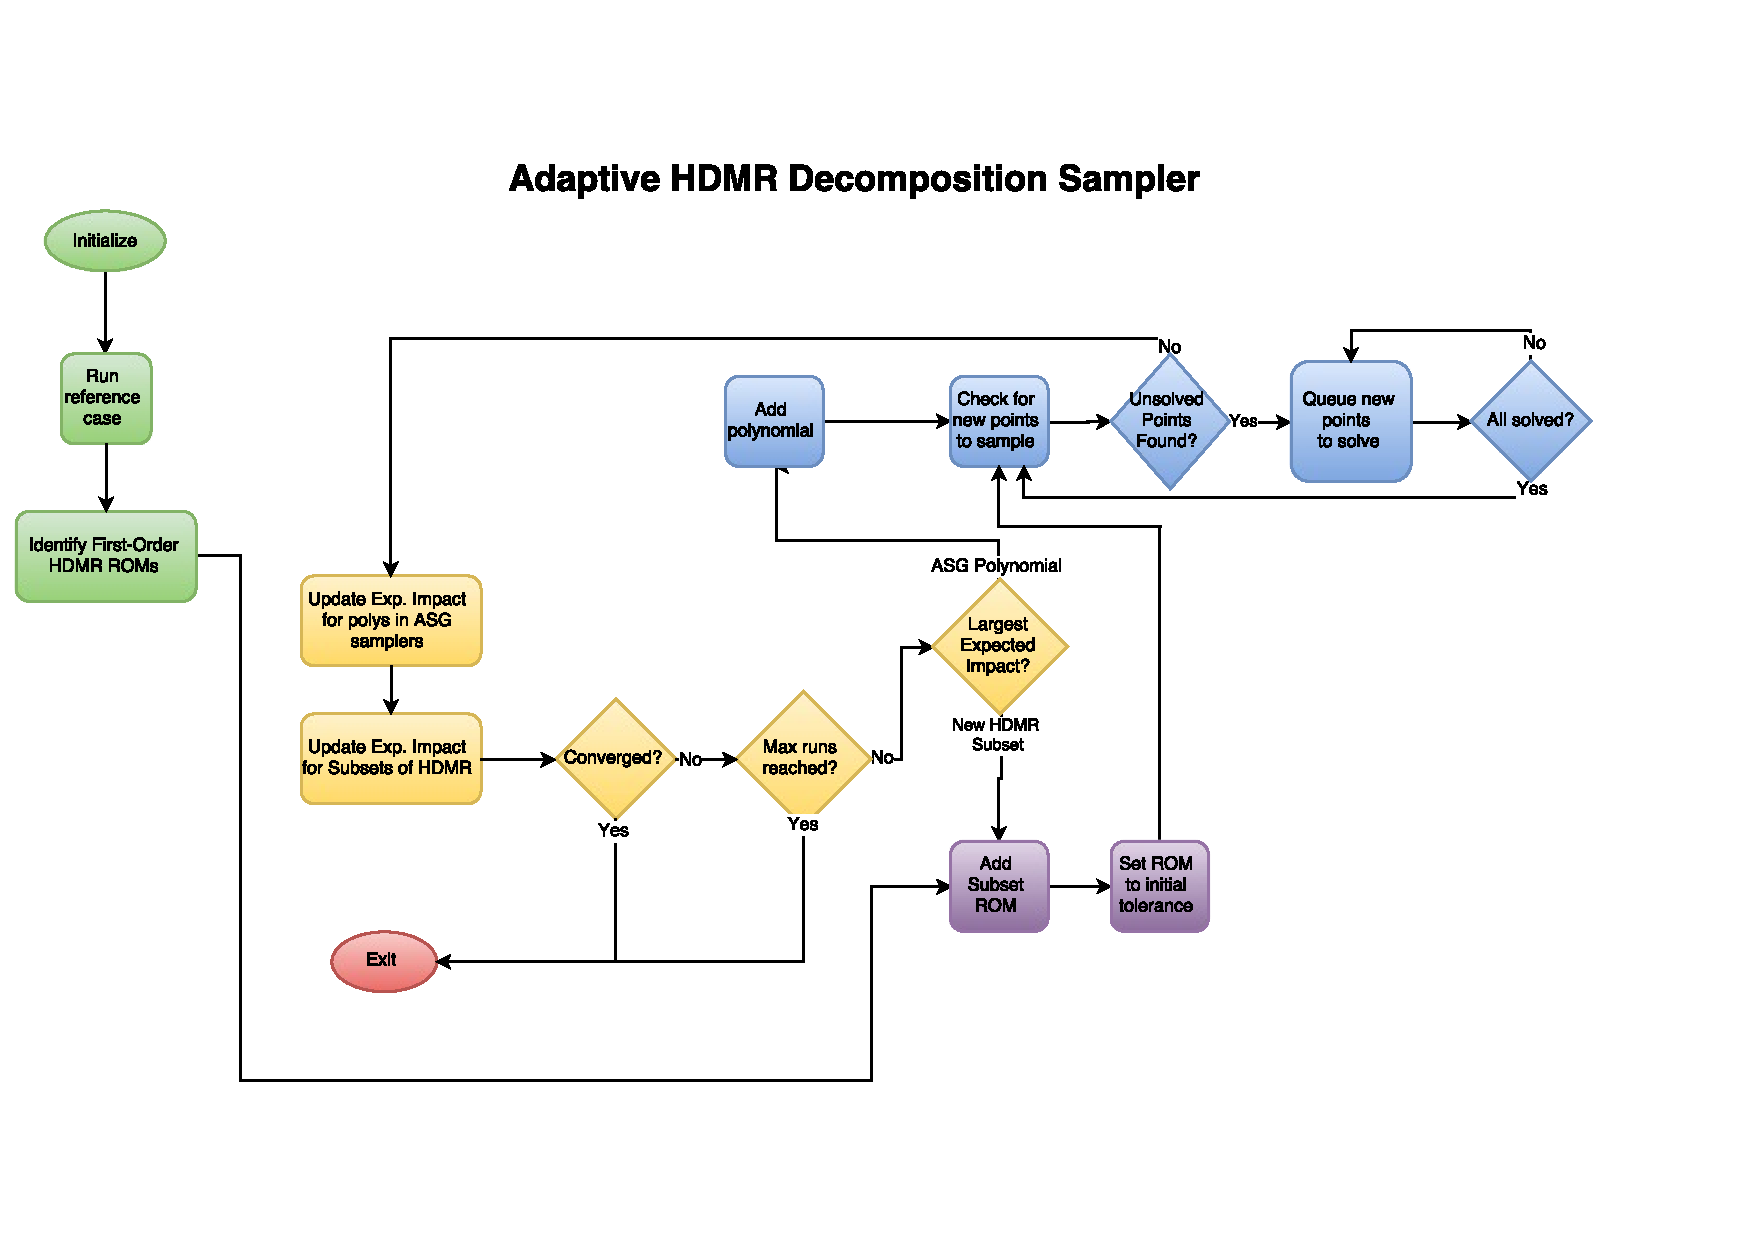
\includegraphics[width=\linewidth]{../graphics/diagram-AHDMR.pdf}
    \rule{35em}{0.5pt}
  \caption{Algorithm for Adaptive HDMR with Adaptive SCgPC}
  \label{fig:flow}
\end{figure}
The green portion is initialization, yellow is convergence, purple is HDMR, and blue is SCgPC.  Particularly of note, at the end of the yellow portion the algorithm must decide whether to add another subset in the HDMR expansion, or add another polynomial to one of the SCgPC expansions.  In order to do this, it needs an \emph{impact factor} to allow quantatative decision making.  A method for calculating an impact factor for both subsets and polynomials is detailed here.

\section{Impact Parameters}
Impact parameters serve two functions: to determine the convergence of the entire algorithm, as well as project the sensitivity of the reduced-order model to uncalculated components of the expansion.  We consider impact parameters for both the subsets of the HDMR expansion as well as polynomials in the SCgPC expansion.

\subsection{HDMR Subset Impact Parameter}
Because the Sobol' sensitivity indices are a direct result of constructing the HDMR expansion, we use these for determining the expected impact of each subset parameter as outlined in Ayres and Eaton's 2015 paper.  Sobol' sensitivity indices are given by
\begin{equation}
S_a \equiv \frac{\text{var}[f_a]}{\text{var}[f(a,b,c,d)]}.
\end{equation}
To predict sensitivity indices for subsets that have not yet been constructed, we use the product of precedent subsets.  For example, the predicted sensitivity $\tilde S_{ab}$ is the product of the actual sensitivities $S_a,S_b$:
\begin{equation}
\tilde S_{ab} \equiv S_a \cdot S_b.
\end{equation}
This estimated sensitivity is used for the expected impact of this index on the total expansion.

\subsection{SCgPC Polynomial Impact Parameter}
Unlike the HDMR subset impact parameter, literature has not provided definitive direction for expected impact parameters.  To recall, the gPC expansion of quantity of interest $G$ (which is a function of $Y=y_1,y_2,y_3$) is given by
\begin{equation}
  G[f](Y) = \sum_{k\in\Lambda} c_k \Phi_k(Y),
\end{equation}
where $\Lambda$ is the set of desired polynomials, $k$ is a multi-index with cardinality equal to that of the uncertainty space, $c_k$ are scalar values, $\Phi_k$ are multidimensional orthonormal polynomials, and
\begin{align}
\Phi_k(Y) \equiv \prod_{n=1}^N \phi_{k_n}(y_n)
\end{align}
where $N$ is the cardinality of the uncertainty space.  The index set $\Lambda$ is constructed adaptively based on the expected impact of successive polynomials.\\

Because of the orthonormality of the polynomials, the variance of this gPC expansion is given by the sum of the square of the coefficients:
\begin{equation}
\text{var}[G(Y)] = \sum_{k\in\Lambda} c_k^2.
\end{equation}
Because of this, we can quantify the relative impact of each coefficient on the total variance by
\begin{equation}
\eta_k = \frac{c_k^2}{\text{var}[G(Y)]}.
\end{equation}
Similar to the Sobol sensitivities, we can approximate the impact of an additional polynomial using its predecessors.  For example, the estimated sensitivity $\tilde\eta_{(3,4,2)}$ of the gPC expansion to the polynomial that's third-order in $y_1$, fourth-order in $y_2$, and second-order in $y_3$ ($k=(3,4,2)$) is dependent on polynomials for $k=(2,4,2), (3,3,2),$ and $(3,4,1)$:
\begin{equation}
\eta_{(3,4,2)}\equiv\frac{c^2_{(3,4,2)}}{\text{var}[G(Y)]}\approx\tilde \eta_{(3,4,2)} = \eta_{(2,4,2)}\cdot\eta_{(3,3,2)}\cdot\eta_{(3,4,1)}.
\end{equation}

\section{Using the Impact Parameters}
When the algorithm comes to the point where it is not converged and needs to either add a polynomial to one of the subset gPC expansions, or add a new subset to the expansion, it makes use of the estimated impact parameters.

The first challenge is comparing polynomial impact parameters from one subset gPC expansion to another.  The second challenge is comparing polynomial impact parameters with new subset impact parameters.  In order to accomodate both, we introduce the global estimated sensitivity parameter for a polynomial within a subset, $\xi^{\text{subset}}_{\text{order}}$, for example, $\xi^{y_1,y_2,y_3}_{(3,4,2)}$.  This global approximate sensitivity parameter is calculated as
\begin{equation}
\xi_{(3,4,2)}^{y_1,y_2,y_3} \equiv \tilde\eta_{(3,4,2)} S_{y_1y_2y_3}.
\end{equation}
The philosophy behind this estimation is to temper the importance of a single polynomial with the importance of that subset.  In essence,
\begin{equation}
\frac{\text{local contribution}}{\text{local variance}}\cdot\frac{\text{local variance}}{\text{global variance}} = \frac{\text{local contribution}}{\text{global variance}}.
\end{equation}
While not perfectly rigorous, it addresses somewhat both comparing the impact of individual polynomials within subsets as well as comparing polynomial contributions to new subset contrubtions.
\subsection{Polynomial-to-Polynomial comparison}
The polynomial comparison between two subsets tests if the global estimated sensitivity of one polynomial in one subset is larger than the global estimated sensitivity of another polynomial from a different subset.  For example,
\begin{equation}
\xi_{(3)}^{y_2} \hspace{5pt}\stackrel{?}>\hspace{5pt} \xi_{(2)}^{y_3},
\end{equation}
or
\begin{equation}
\tilde\eta_{(3)} S_{y_2}\hspace{5pt}\stackrel{?}>\hspace{5pt} \tilde\eta_{(2)} S_{y_2}.
\end{equation}
If the impact $\tilde\eta_{(3)}$ on $G(y_2)$ is the same as the impact $\tilde\eta_{(2)}$ on $G(y_3)$, then the most impactful polynomial globally will by determined by the Sobol sensitivity of that subset.  Conversely, if the Sobol sensitivities of the two subsets are identical, then the global impact will be decided by the impact of the polynomial on that subset.
\subsection{Polynomial-to-Subset comparison}
This test is somewhat more difficult to compare without beginning construction of the unknown subset; however, constructing all unknown subsets is undersirable due to the expense and possible lack of gain.  Using the global estimated sensitivity parameter to compare to the estimated Sobol sensitivity gives some insight as to which may be more impactful to the overall HDMR expansion.  For example, in a set where the subset has been constructed for all first-order Sobol subsets but not second-order subsets, the following check might be made for greatest overall impact:
\begin{equation}
\xi_{(3)}^{y_2} \hspace{5pt}\stackrel{?}>\hspace{5pt} \tilde S_{y_1y_3},
\end{equation}
or
\begin{equation}
\tilde\eta_{(3)} S_{y_2}\hspace{5pt}\stackrel{?}>\hspace{5pt} S_{y_1}S_{y_3}.
\end{equation}
There are three cases to consider that will yield some perspective into the performance of this inequality.  These cases compare the expected Sobol sensitivity $\tilde S_{y_1y_3}$ with the partially-converged Sobol sensitivity $S_{y_2}$.\\

If $S_{y_2} = \tilde S_{y_1y_3}$, because $\tilde\eta$ is strictly less than one, the algorithm will prefer to add the new subset.\\

If $S_{y_2} < \tilde S_{y_1y_3}$, there is little sense improving the resolution of the existing subset until the new subset is added.\\

If $S_{y_2} < \tilde S_{y_1y_3}$, however, it entirely depends on $\tilde\eta$.  If the local polynomial impact is quite small, the algorithm is likely to choose to add the subset instead of continuing to resolve the existing subset.  If, however, the expected sensitivity of the new subset is very small, the algorithm will likely resolve the existing subset instead of adding the new subset.\\

\subsection{User-input Control}
One way to introduce a controlling mechanism to prefer either subset resolution or addition of more subsets is by adding an exponential parameter $\alpha$ to the global estimated sensitivity parameter.  For example,
\begin{equation}
(\tilde\eta_{(3)})^\alpha (S_{y_2})^{2-\alpha} \hspace{5pt}\stackrel{?}>\hspace{5pt} (\tilde S_{y_1y_3})^{2-\alpha}.
\end{equation}
We allow $\alpha$ to range from 0 to 2.  When $\alpha$ is zero, no information from the local polynomial impact is considered, and only Sobol sensitivity of subsets is considered.  Because the estimated sensitivity of any new subset is always smaller than all of its predecessors, this will always choose the most impactful existing subset to add a polynomial to, no matter how resolved it already is.  In the other extreme, when $\alpha$ is two, the local impact term becomes quite small, while the adjusted impact parameter for a new subset is always unity.  In this case, the algorithm will always decide to add a new subset and not resolve any existing subsets.\\

Both extreme cases are not ideal; however, the range of values between them serve as a way to prefer resolving polynomials ($\alpha<1$) or prefer adding subsets ($\alpha>1$).
\end{document}